%%
\chapter{Domain modeling in Eclipse Modeling Framework}
\label{chapter:emf}
%%

In this chapter the creation of initial artifacts is presented: domain models and graph patterns.
Domain modeling is an essential part of our framework, as the domain model defines the structure of the runtime live model, and affects the whole process. 
After the domain model is known, graph pattern can be specified, which will be used later in runtime analysis.
In the framework domain modeling are technologically backed up by EMF (Eclipse Modeling Framework), 
while graph pattern definition and processing are provided by \viatra{}.

\section{Eclipse Modeling Framework}


\begin{figure}
	\begin{center}
		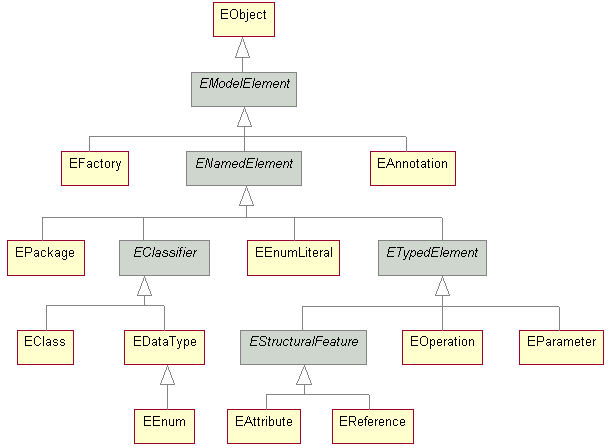
\includegraphics[width=0.5\textwidth]{figures/EcoreHierarchy.png}
		\caption{Hierarchy of Ecore elements \cite{ecore-package} }
		\label{fig:ecore-hierarchy}
	\end{center}
\end{figure}

\begin{figure}
	\begin{center}
		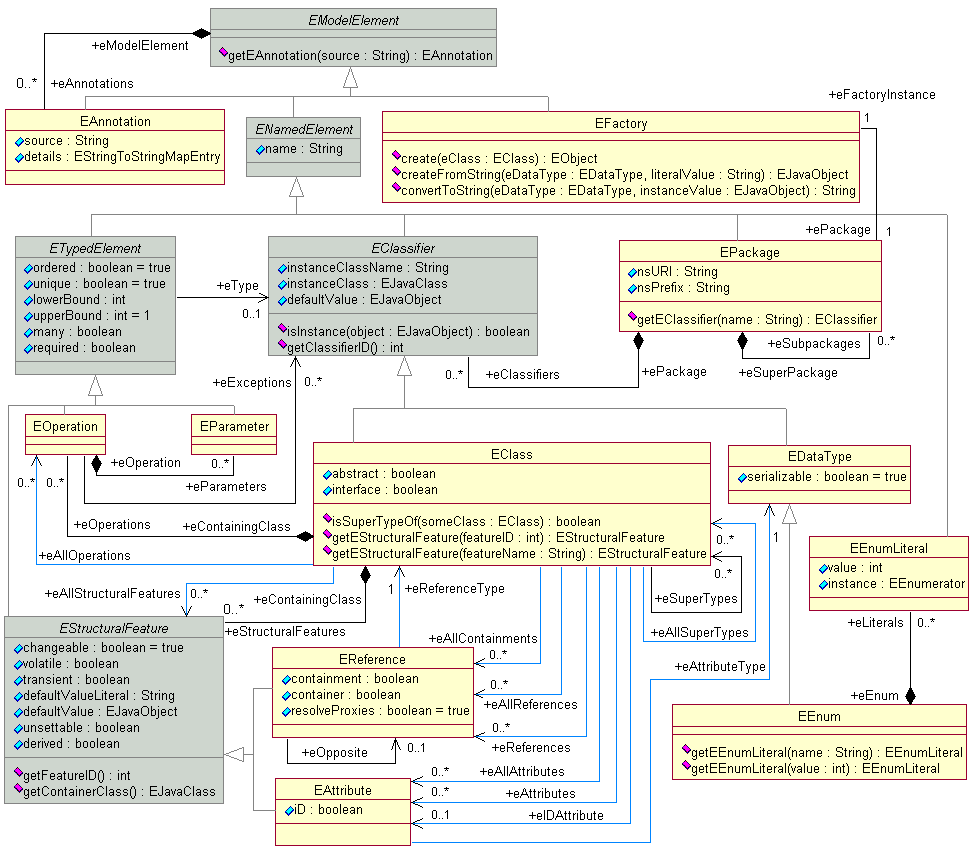
\includegraphics[width=\textwidth]{figures/EcoreRelations.png}
		\caption{Relations between Ecore elements \cite{ecore-package} }
		\label{fig:ecore-relations}
	\end{center}
\end{figure}

Eclipse Modeling Framework (EMF) is an Eclipse-based technology, which provides tools for model-based development: 
Ecore \cite{ecore-package} for metamodeling, and various tools like java code generation from Ecore models, etc.

Ecore metamodeling is highly similar to defining class diagrams in UML, however, 
Ecore is more suitable for data and structural modeling: Interfaces are not a part of it, even though it can be substituted by abstract classes, as multiple inheritance is supported.

The hierarchy of Ecore elements can be seen in \autoref{fig:ecore-hierarchy}, while its structure in \autoref{fig:ecore-relations}
EObject is a base for everything, and its main purpose to define the containment hierarchy of the model. 
EObjects can contain each other in a strict tree structure, circular containments are not permitted.
EModelElement expands EObject by giving the possibility to annotate them.

An Ecore model contains packages (\texttt{EPackage}). 
Packages have a namespace URI (\texttt{nsURI}), which can be used to refer to the package in other contexts e.g.\ Viatra graph pattern definition.
Packages can contain other subpackages, classes (\texttt{EClass}), enumerations (\texttt{EEnum}), and data types (\texttt{EDataType}).

Classes have structural features: references and attributes (\texttt{EStructuralFeature}, \texttt{EReference}, \texttt{EAttribute}); also they have operations (EOperation).
References and attributes have multiplicity, defining their lower and upper bound is also possible.
ECore also provides tools to define containment hierarchy in the domain model itself: a reference can be a containment or a containing reference considering the direction of the edge. 
Two-way navigation can be achieved by defining two references as each other's EOpposite. A reference cannot be the \texttt{EOpposite} of itself, but its not a problem in most of the cases (e.g.\ \texttt{Human} class and \texttt{Spouse} reference). 

Multiple inheritance is supported for classes: eSuperTypes refers to direct base classes, and eAllSuperTypes for all transitively inherited base classes.

Besides classes, packages can contain enumerations and data types. 
Basic data types -- like EString, EInt, EBoolean etc.\ -- are defined by EMF, so it is almost never necessary to define others.
Enumerations are consists of EEnumLiterals. 
EEnumLiterals are identified by a unique integral value.
The name of the literal is encapsulated in its EEnumerator instance.


\section{Metamodel from the case study}

The metamodel of our case study is depicted in \autoref{fig:unified-mm}.
containment edges are marked by a black diamond at the container object.
The \texttt{MoDeS3ModelRoot} is the root of the containment hierarchy, only one. Computing units are represented by the \texttt{ComputingModule} class. \texttt{DomainElement} is the base class for all the classes representing an element of the railway systems. \texttt{Train} represents the trains, The railways are consisted of the instances of \texttt{RailRoadElement}. A \texttt{RailRoadElement} divides between a \texttt{Turnout} with \texttt{straight} and \texttt{divergent} track. \texttt{Segments} are simple railway segments with one or two neighbors. A \texttt{connectedTo} reference exists between two rail road elements, if the train can travel from one to the other.

\begin{figure}[H]
	\begin{center}
		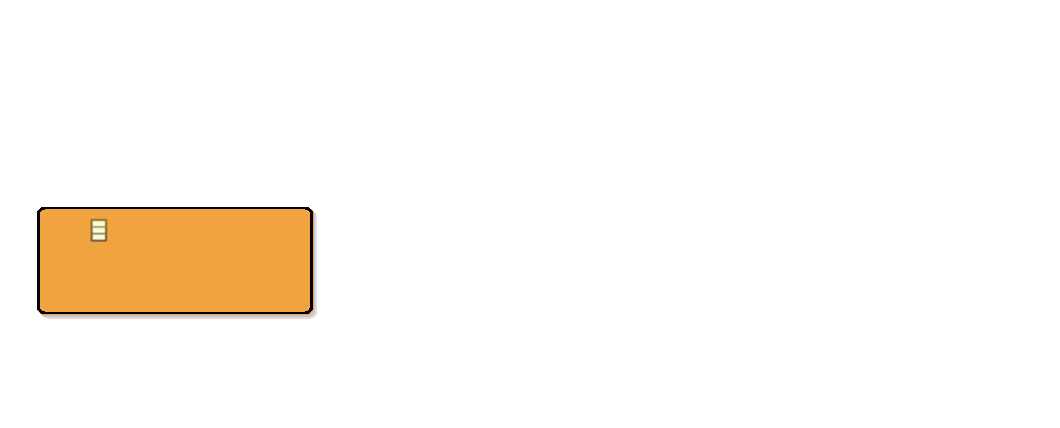
\includegraphics[width=\textwidth]{figures/unified-mm.pdf}
	\end{center}
	\caption{Metamodel from the case study}
	\label{fig:unified-mm}
\end{figure}


